\subsection{Convention for numbering interpolatory vertices}
\label{impl-gmsh-numbering-convention}

This section discusses the different conventions for numbering interpolatory vertices for \textit{Lagrange}-based curvilinear entities. The convention used in \textit{Lagrange} interpolation is placing of the interpolatory vertices on a regular grid over the entity, the number of vertices on each edge corresponding to the interpolatory order minus 1, i.e. 2 points to define linear edge, 3 to define quadratic and so on. The convention used in \textit{} can be called \textit{Sorted Cartesian} indexing, and is described by the following vertex enumeration algorithm.

\begin{mybox}
\begin{lstlisting}
for (z=0 to 1, y=0 to 1-z, x=0 to 1-z-y) { vertex(x,y,z); }
\end{lstlisting}
\end{mybox}


\noindent
Instead, the \gmsh{} community uses the a recursive convention

\begin{enumerate}
	\item First number all corners, then all edges, then all faces, then the vertices interior to the element element
	\item Inside an edge, vertices are numbered sequentially from starting to finishing corner
	\item Inside a face, a new triangle is defined recursively from the outer-most interior vertices, with the same order as the original triangle
	\item Inside an element, a new element is defined recursively from the outer-most interior vertices, with the same order as the original triangle
	\item For a triangle, the order of edges is $(0,1)$, $(1,2)$, $(2,0)$. (in 2D)
	\item For a tetrahedron, the order of edges is $(0,1)$, $(1,2)$, $(2,0)$, $(3,0)$, $(3,2)$, $(3,1)$.
	\item For a tetrahedron, the order of faces is $(0, 2, 1)$, $(0, 1, 3)$, $(0, 3, 2)$, $(3, 1, 2)$, including orientation
\end{enumerate}

\noindent
We are still looking for a nice algorithm to analytically map between both conventions for arbitrary order entities. For now, we hard code the  \textit{GMSH} to  \textit{Dune} map for simplex geometries up to order 5. The following table contains the Dune-notation vertex indices corresponding to ascending \textit{GMSH} vertex index

\begin{figure}[H]
    \centering
    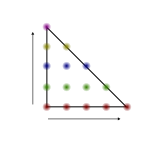
\includegraphics[scale=1]{images/vertex-grid-dune}
    \caption{Sorted Cartesian interpolatory vertex enumeration}
    \label{fig:appendix:gmsh:enumeration:dune}
\end{figure}

\begin{figure}[H]
    \centering
    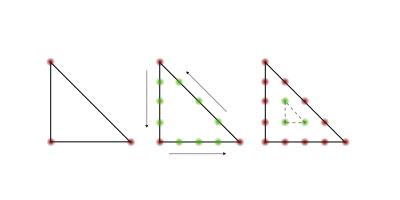
\includegraphics[scale=1]{images/vertex-grid-gmsh}
    \caption{ \textit{GMSH} recursive interpolatory vertex enumeration}
    \label{fig:appendix:gmsh:enumeration:gmsh}
\end{figure}


\begin{mybox}
\begin{itemize}
	\item Triangle Order 1: \{0, 1, 2\}
	\item Triangle Order 2: \{0, 3, 1, 5, 4, 2\}
	\item Triangle Order 3: \{0, 3, 4, 1, 8, 9, 5, 7, 6, 2\}
	\item Triangle Order 4: \{0, 3, 4, 5, 1, 11, 12, 13, 6, 10, 14, 7, 9, 8, 2\}
	\item Triangle Order 5: \{0, 3, 4, 5, 6, 1, 14, 15, 18, 16, 7, 13, 20, 19, 8, 12, 17, 9, 11, 10, 2\}
	
	\item Tetrahedron Order 1: \{0, 3, 1, 2\}
	\item Tetrahedron Order 2: \{0, 7, 3, 4, 9, 1, 6, 8, 5, 2\}
	\item Tetrahedron Order 3: \{0, 11, 10, 3, 4, 17, 14, 5, 15, 1, 9, 18, 12, 16, 19, 6, 8, 13, 7, 2\}
	\item Tetrahedron Order 4: \{0, 15, 14, 13, 3, 4, 25, 27, 19, 5, 26, 20, 6, 21, 1, 12, 28, 29, 16, 22, 34, 31, 24, 32, 7, 11, 30, 17, 23, 33, 8, 10, 18, 9, 2\}
	\item Tetrahedron Order 5: \{0, 19, 18, 17, 16, 3, 4, 34, 39, 36, 24, 5, 37, 38, 25, 6, 35, 26, 7, 27, 1, 15, 40, 43, 41, 20, 28, 52, 55, 46, 33, 53, 49, 30, 47, 8, 14, 45, 44, 21, 31, 54, 51, 32, 50, 9, 13, 42, 22, 29, 48, 10, 12, 23, 11, 2\}
\end{itemize}
\end{mybox}